\documentclass[11pt]{article}
\usepackage{fullpage}
\usepackage{array}
\usepackage{graphicx}
\usepackage{amssymb, amsmath}
\usepackage{hyperref}
\usepackage[labelfont=bf]{caption}

\begin{document}


\title{\textbf{Tabulation of Chemical Source Terms for Turbulent
    Combustion Simulations}}

\author{Emmet Cleary: emcleary@princeton.edu \and Daniel Floryan:
  dfloryan@princeton.edu \and Jeffry Lew: jklew@princeton.edu \and
  Bruce Perry: bperry@princeton.edu \and Emre Turkoz:
  eturkoz@princeton.edu} 

\date{21 November 2014 }
\maketitle

\section{Introduction}
Turbulent combustion simulations require closure of chemical source terms (reaction rates). This is not trivial, as the chemical source terms follow highly nonlinear Arrhenius kinetics and can depend on numerous stiffly-coupled chemical reactions. One approach, rather than evaluating these terms during simulations, is to calculate a set of thermochemical states \textit{a priori} and use these when solving conservation equations. When combined with flamelet models\footnote{Pierce \textit{et al.}, J. Fluid Mech. (2004) vol. 504, pp. 73-97.}, chemical source term tabulation greatly facilitates large eddy simulations (LES) of turbulent reacting flows.

The challenge with these tabulation methods is knowing how to identify
each term as needed.  This is done by tabulating source terms against
a predetermined variable. The trick is to find a bijective mapping
between a single progress variable and the thermochemical
states. Temperature is the most obvious one: the more a reaction
proceeds, the more heat is released. However, filtering the energy
conservation equation for LES leads to a closure problem. It is much
simpler to filter species conservation equations, but a single
chemical species is usually insufficient to identify the
thermochemical state uniquely. Rather, one must take a linear
combination of several species, called a progress variable, to define
a mass-based conservation equation that is suitable for turbulent
combustion simulations. Once a progress variable is chosen, the
thermochemical states can be sorted, convoluted with a probability
density function (PDF) to calculate filtered quantities for LES, and
interpolated as needed to generate a table of chemical source terms (a
“chemtable”) on a predefined grid.

Our project will use outputs from an existing research code called
FlameMaster to facilitate and automate the selection of progress
variables. Our project will also process output data from FlameMaster
to create a chemtable through sorting based on the selected progress
variable, convoluting, and interpolating. A variety of interpolation
schemes, integration methods, and PDFs will be incorporated into the
code to ensure that it is easily adaptable. The automated selection of
progress variable has not been implemented in any existing
code. Furthermore, although there exists code that can create
chemtables after the progress variable has been defined, it lacks
generality and must be rewritten or substantially modified when
requirements for the chemtable change. A modular program for this task
with well-defined interfaces will significantly improve the usability
of the chemtable code.

\section{Architecture}
Our project consists of two related parts: determining the best
progress variable (Fig.~\ref{fig:flow1}) and generating the chemtables
(Fig.~\ref{fig:flow2}). Our program will be based in C++. SWIG will be
used to interface the C++ functions to a Python wrapper that includes
the user interface. The following tools will be used during software
development:

\subsection{Progress Variable}
As shown in Fig.~\ref{fig:flow1}, inputs to the progress variable
section of our program include a text input file containing the user’s
selection of options to be used during run time and many combustion
data files containing thermochemical state information. The final
output is the best progress variable, which is passed to the table
generation section of our program in Fig.~\ref{fig:flow2}. Detailed
descriptions of the processes in Fig.~\ref{fig:flow1} are below.

\begin{enumerate} 
\item Input files contain a user-specified stoichiometric mixture
  fraction value, a user-specified list of species mass fractions, and
  a set of full thermochemical states represented as columns of
  temperature, species mass fraction, and chemical source terms in
  mixture fraction space. All combinations of mass fractions in the
  user-specified list are candidates for the progress variable.

\begin{figure}[h]
  \centering
  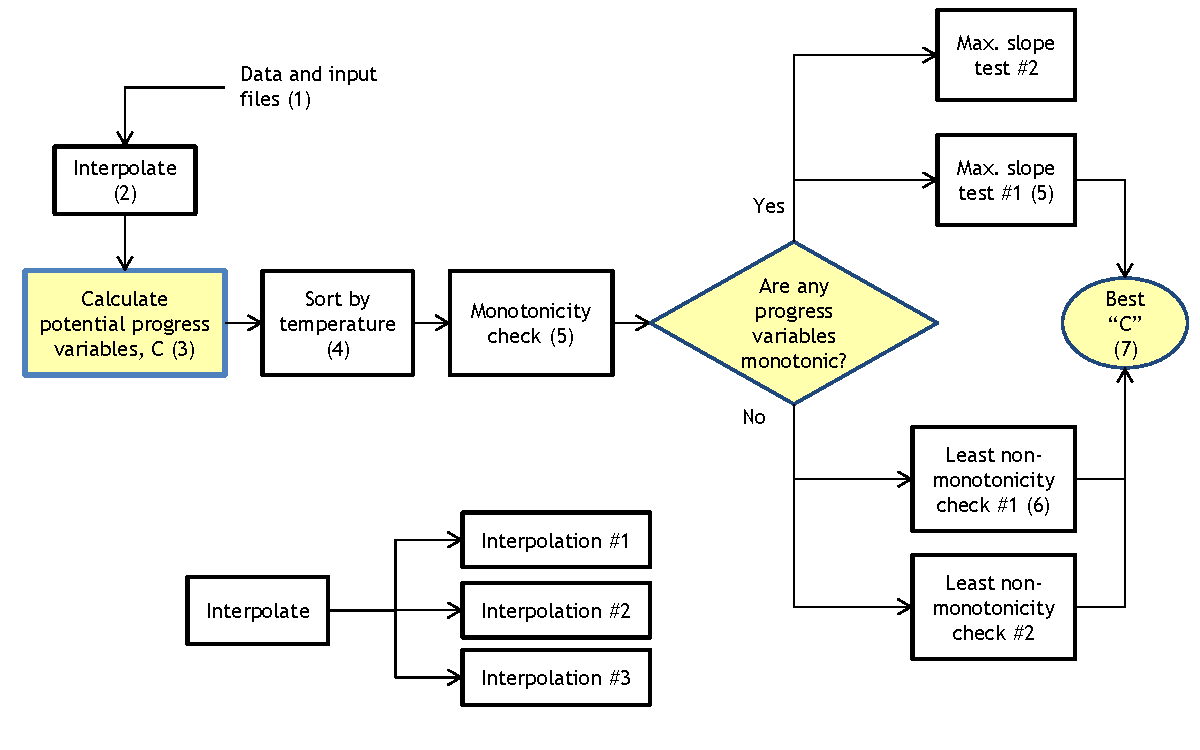
\includegraphics[width=\textwidth]{diagram_1_v4.pdf}
  \caption{\label{fig:flow1}Flowchart depicting key steps in
    determining the best progress variable. Colored boxes indicate
    tasks that will be accomplished in Python and white blocks
    indicate tasks that will be accomplished with C++ functions.}
\end{figure}

\item Python code exports two rows from each data file to be
  interpolated at the stoichiometric mixture fraction.
\item Python code calculates all progress variable candidates at these
  interpolated values.
\item C++ code sorts all progress variables by the stoichiometric
  temperature through various sort functions, generating arrays of
  temperature and all progress variables. These arrays are the only
  data used for the rest of this section.
\item All progress variables are tested for monotonicity with
  temperature in C++ code.
\item Monotonic progress variables will be ranked by various tests,
  \textit{e.g.} an average slope test.
\item If no monotonic progress variables exist, the variables will be
  tested to pick the one that is least non-monotonic, \textit{e.g.}
  monotonic over the greatest range.
\item The best progress variable will be sent to the table generation
  section.
\end{enumerate}




 
\subsection{Table Generation}
The table generation portion of our project is shown in
Fig.~\ref{fig:flow2}.  Inputs include the best progress variable from
the previous section, thermochemical states (data files), and a text
input file containing the user's selection of options and chemtable
grid.  The final output of this part of the code is a chemtable, which
can be fed into computational fluid dynamic codes.  Detailed
descriptions of the processes in Fig.~\ref{fig:flow2} are below.


\begin{enumerate}
\item The input data files are the same inputs used for the progress
  variable selection. The best progress variable, as determined by the
  processes depicted in Fig.~\ref{fig:flow1}, is also an input.
\item Progress variable is calculated for each data file and
  interpolated to find the value at the stoichiometric mixture
  fraction $C_{st}$. Various interpolation schemes will be used in the
  required sections of the program.
  % These interpolation schemes are conducive to polymorphism -
  % specific styles of interpolation will be employed as classes which
  % inherit from an abstract interpolation class.
  User selection of the interpolation methods for each process will be
  determined from the text input file which will contain the chosen
  scheme.
\item The data files will be sorted by the stoichiometric progress
  variable.
  % , again using inheritance and polymorphism for the sorting
  % functions.
  The algorithm used will be read from the text input file.
\item Numerical integration schemes will be used in the convolution
  step.
  % Like interpolation and sorting, these numerical integration
  % schemes exploit inheritance and polymorphism.
  Again, the numerical integration scheme is determined by the user in
  the text input file.
\item The progress variable will be convoluted with PDFs. The user
  will specify which PDF to use for convolution.
  % The implementation will be polymorphic and the PDF to be used will
  % be specified in the text input file.
  The output will be an array of values to be passed to the next
  process.
\item These values will be interpolated onto a table (grid) that is
  specified by the text input file.  This is the chemtable that will
  be the final output of our program.
\end{enumerate}
\begin{figure}[h]
  \centering
  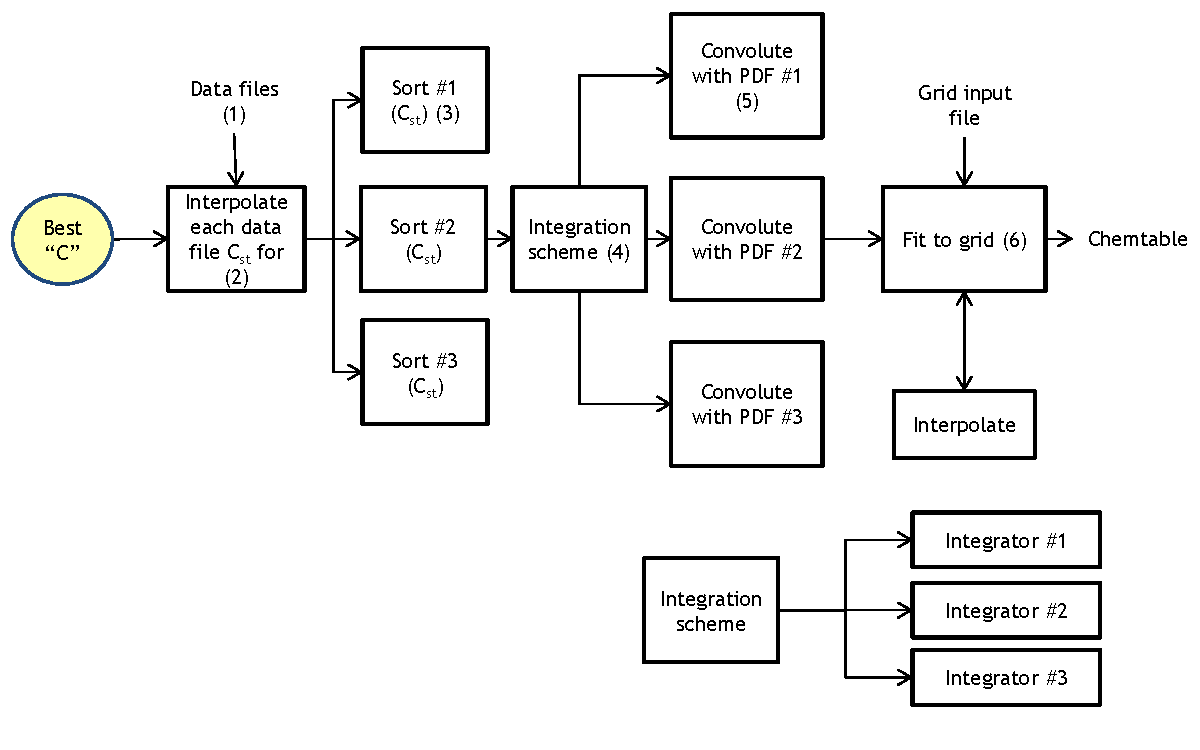
\includegraphics[width=\textwidth]{diagram_2_v4.pdf}
  \caption{\label{fig:flow2}Flowchart depicting key steps in
    generating from the chemtables, using the definition of progress
    variable determined by the first section of code. All functions
    for this section of the program will be written in C++, but as
    with the progress variable section these functions will be called
    from a Python program that provides the user interface.}
\end{figure}

\subsection{Implemented Schemes/PDFs}
Several of the steps in both section sof the program are conducive to
polymorphism --- for example, interpolation schemes will be employed
as classes which inherit from an abstract interpolation
class. Multiple integration methods, sorting schemes, and PDFs will be
implemented in a similar manner. Here are some examples of the
polymorphic classes that we will use in our codes:

\subsubsection{Sort}
\begin{itemize}
\item Bubble sort 
\item Binary sort
\item C++ Standard Library
\end{itemize}

\subsubsection{Integration}
\begin{itemize}
\item Trapezoid method
\item Simpson's rule
\item Gaussian quadrature
\end{itemize}

\subsubsection{Interpolation}
\begin{itemize}
\item Linear
\item Cubic spline
\item Bilinear
\end{itemize}

\subsubsection{Probability Density Function}
\begin{itemize}
\item Delta function
\item Beta distribution
\item Most probable distribution
\end{itemize}

\subsection{External Functions}

We will use the following outside functions and packages to facilitate
the development of our software:
\begin{enumerate}
\item C++ Standard Library
\item Numpy - matrix and vector calculations in Python
\item Matplotlib - contour plots of chemtable results
\item SWIG - interface between Python and C++
\item FlameMaster (existing research software) - our code will not
  interact with FlameMaster, but the data files generated by
  FlameMaster will serve as inputs to our code
\end{enumerate}

\section{Milestones}
\textbf{Prototype - 12/5/2014}: This version will have one element
from each step working separately. Mathematical routines will be coded
in C++. The two sections of the code will be developed separately. The
tasks will be divided as follows:
\begin{itemize}
\item Interface between functions (All)
\item Interpolation routines (Daniel)
\item Sorting algorithms (Emre, Jeffry)
\item Monotonicity check and maximum slope tests (Bruce, Jeffry)
\item Integration schemes (Emmet, Daniel)
\item Probability density functions (Emmet)
\item I/O text processing. (Emre, Bruce)
\end{itemize}

\noindent \textbf{Alpha version - 12/12/2014}: This version will
include one element from each step at the presented pipeline and will
be able to run with a simple configuration:
\begin{itemize}
\item Preliminary Python wrapper implemented using SWIG to allow
  for some user interaction (Emre, Emmet)
\item One routine from each step (1 interpolator, 1 sorting algorithm,
  the basic monotonicity check, maximum slope check, 1 integration
  scheme along with 1 PDF) will be implemented in C++ (All)
\item The link between the progress variable selection and chemtable
  generation sections will be implemented with Python (Daniel,
  Jeffry)
\item Fully-functional program that works on well-behaved data
  sets (All)
\item Basic plotting capability will be incorporated for visualization
  of the preliminary results.  (Bruce)
\end{itemize}

\noindent \textbf{Beta version - 01/6/2015}: This will be final
version.  Each group member will extend their own sections from the
prototype and alpha version. The beta version will contain:
\begin{itemize}
\item Fully-operational Python wrapper allows for autonomous and
  interactive use
\item Implementation of remaining function for interpolation, least
  non-monotonicity checking, integration, PDFs, and sorting
\item Fully-functional program that works on real FlameMaster output
  data
\item Interactive and advanced plotting capabilities will be
  incorporated for visualization
\item Error-checking functionality
\item Speed of key functions will be optimized.
\end{itemize}


\section{Risks and Open Issues}

The runtime of our code may be an issue for large data sets and for
the cases that require large number of progress variable
candidates. Also for our research purposes, the data sets may consist
of hundreds of files. If runtime turns out to be an issue, we
may consider implementing parallelization using OpenMP.

% One potential issue in completing the alpha version within the given
% project time constraints. The groundwork for our project must be
% laid with the completion of the alpha version.

Identifying a truly bijective mapping between progress variable and
thermochemical state is among the most challenging and subjective
parts of turbulent combustion simulations using flamelet models. In
fact, a bijective mapping may not even exist. This poses a risk, not
that the program will crash, but that the program will give incorrect
output. Furthermore, even perfectly monotonic progress variables may
have wildly varying slopes over temperature, so the highest average
slope may not necessarily give the best progress variable. For our
project to be incorporated into research codes it must still be able
to deal with these challenging situations. In the worst cases, this
can only be dealt with through plotting numerous graphs and requiring
the user to visually determine the best progress variable. Regardless,
our code will still greatly facilitate this process.

Both sections of our project are independently capable of improving
current codes. Even if one is not successful, our project will still
provide a useful tool for turbulent combustion simulations. And due to
the modular structure of our project, even if one component cannot be
completed, the remaining portions will not be affected by this
problem. Furthermore, the modular structure of our project allows us
to develop the various components in parallel and rapidly iterate
through versions of our code.

% Risks
% -- handling cases where monotonic progress variables are not possible
% -- ????




\end{document}

 
